\section{Introduction}

Suppose the only training data for a household robot is a handful of egocentric recordings: one person, one home, one bucket, one counter. A policy trained on the clip in Fig.~\ref{fig:teaser}a learns to wipe that counter; change the laminate to blue or swap the bucket and nothing in the data says the task is the same. Vision-language-action (VLA) models such as RT-2~\cite{rt2}, OpenVLA~\cite{openvla} and $\pi_0$~\cite{pi0} avoid the problem with demonstration sets of hundreds of thousands of episodes~\cite{oxe}, much of which exist to cover appearance rather than new skills. Recording that diversity by hand is the slow part: our own material is 8 recordings, about 80 minutes of footage.

\begin{figure}[t]
\centering
\begin{subfigure}{0.33\linewidth}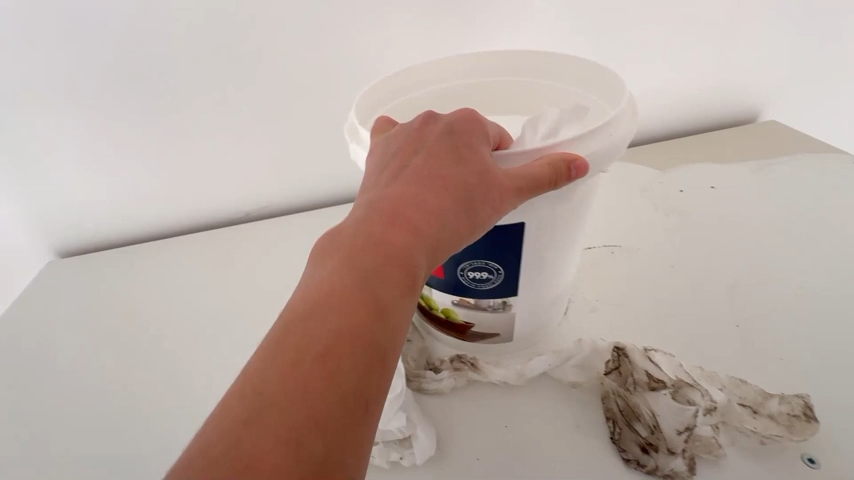
\includegraphics[width=\linewidth]{s03_original.png}\caption{what we started with}\end{subfigure}\hspace{2mm}
\begin{subfigure}{0.33\linewidth}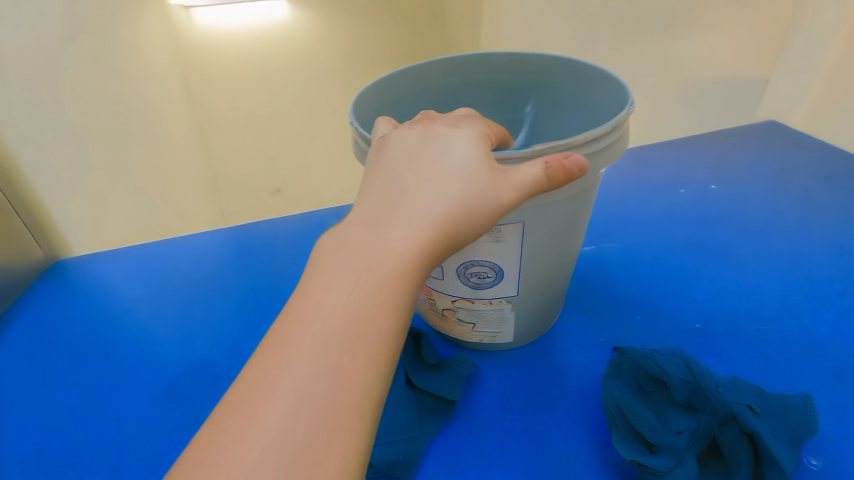
\includegraphics[width=\linewidth]{s04_created.png}\caption{what we created}\end{subfigure}
\caption{The running example. (a) A real clip: a person wiping a counter with a bucket and rags. (b) The variant rendered when asked to change only the countertop to blue. Counter color, hand pose, bucket geometry and motion are as intended; the beige wall, blue rags and bucket, and new ceiling light were not asked for.}
\label{fig:teaser}
\end{figure}

The existing shortcuts each give up something. Domain randomization~\cite{tobin2017} perturbs colors and textures with no notion of the scene, so it will give a cleaning bucket a texture no bucket has. Generative augmentation with image diffusion models~\cite{rosie,genaug} fixes plausibility for single frames but does not hold hands and objects steady across 60 frames. Structure-conditioned video models~\cite{gen1,controlnet} can restyle a whole clip, and NVIDIA's Cosmos family~\cite{cosmos2025} packages this for physical AI, but none of them decide what should change in a clip and what must stay fixed. We chain existing models so that a reasoning step makes that decision and a guided renderer carries it out (Fig.~\ref{fig:teaser}b). We set out to support three claims and report how far the evidence goes: that a pipeline on Cosmos can take a small real dataset to thousands of candidate clips; that appearance changes work for simple scenes and break down for cluttered scenes and action-level changes, which we measure; and that reasoning about the scene yields task-grounded rather than random variations, which holds by construction and still awaits a baseline. The open question is whether appearance diversity alone makes a policy more general, or whether action generation has to be solved first.
